The final paper does not focus on GWAS, but rather on the predictive value of the LT-FH++ phenotype as an alternative to the conventional binary family history variable in prediction models. In epidemiology, family history is a well-known and powerful predictor that has been used to improve prediction models of complex phenotypes such as mental disorders, suicide, and heart disease. As the intension is to provide an estimate of an individual's liability for a given disorder before getting an actual diagnosis, we will not consider the case-control status of the index person, but only the family members. In many ways this is similar to the purpose of the PRS and how it is currently being used to screen individuals for disorders. However, instead of using the individual's genotypes to acquire an aggregate genetic risk score, we will use the family history to estimate a liability. 

\subsection{Real-World Analysis}

\begin{wrapfigure}{O}{10cm}
	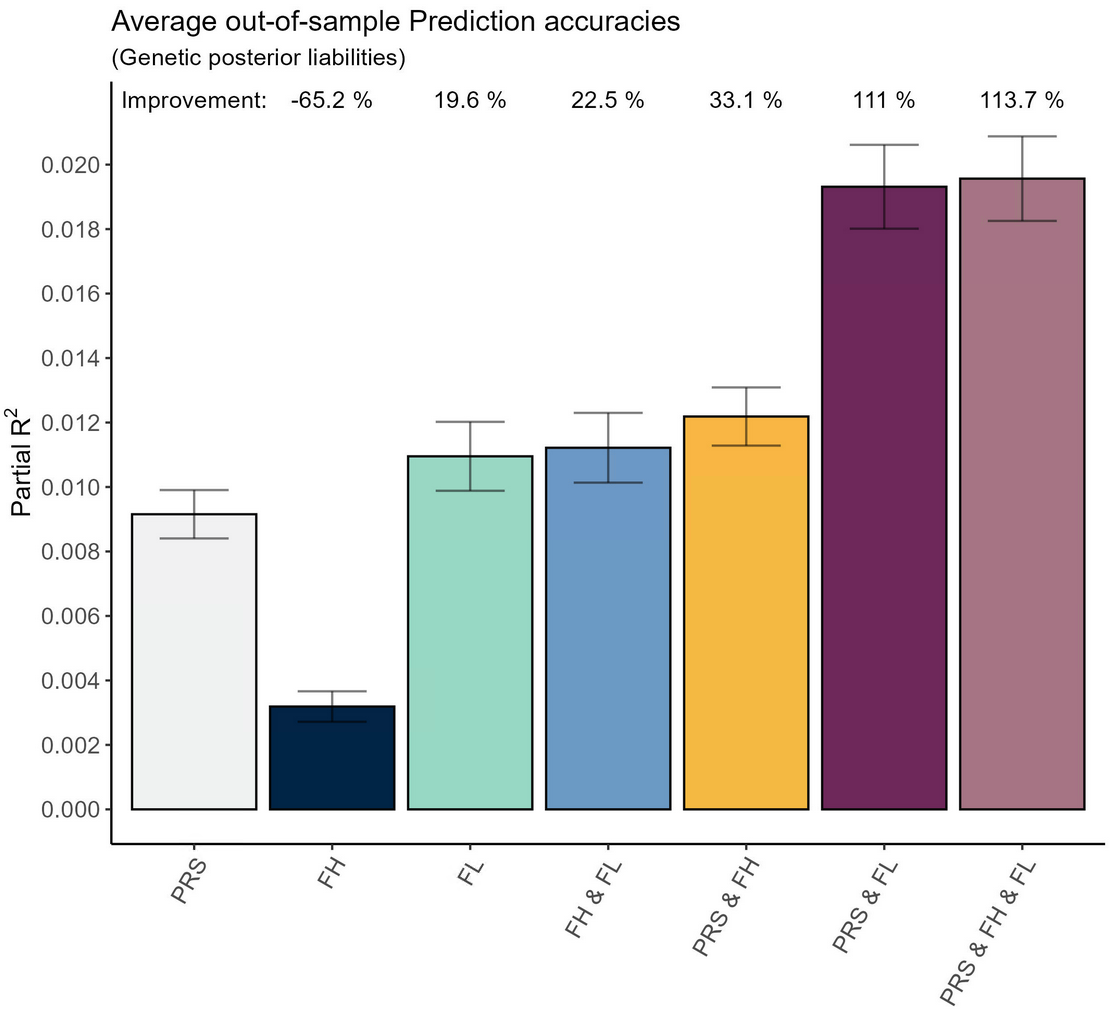
\includegraphics[width=10cm]{results/avg_partial_prediciton_accuracies_noED.png}
	\caption[Average out of sample prediction across $ 8 $ disorders]{
		\sl Average partial $ R^2 $ across $ 8 $ disorders with various prediction models. We excluded eating disorders from the average, as hardly any family history was present for these disorders. The base model includes age, sex, and $ 20 $ PCs. \textit{PRS} refers to the base model with the PRS included as well. \textit{FH} refers to the base model with the binary family history, and \textit{FL} refers to the LT-FH++ variable. Combinations of these variables are presented as \textit{PRS} \& \textit{FH} for the model with PRS and the binary family history variable etc..}
	\label{fig:paper3:predictionResults}
\end{wrapfigure}

We will consider a base model that contains the index person's sex, age, and $ 20 $ PCs. We will add additional predictors to the base model and assess the additional predictive value of each predictor. We will use the partial $ R^2 $ as a measure of predictive value. From the additional predictors and combinations of them, we can derive the best family history variable and the best overall model. We will consider the PRS for a given disorder, as well as a binary family history indicator or the LT-FH++ phenotype (but with the index person's status removed). We present the results in \cref{fig:paper3:predictionResults}. We calculated the average partial $ R^2 $ across $ 8 $ phenotypes available to iPSYCH, but we left out eating disorders, as there were almost no family history available. We find that the LT-FH++ phenotype provided a $ 19.6\% $ increase over the the PRS model, while the binary family history variable had a predictive value $ 65.2\% $ lower than the PRS model. Of the models with only two predictors, the best model was the one with the PRS and LT-FH++ phenotype predictors. They had an average partial $ R^2 $ of $ 111\% $ across the $ 8 $ disorders, resulting in a partial $ R^2 $ value that is close the sum of each predictor. The model with both family history variables had almost the same predictive value as the model with only the LT-FH++ variable, indicating that most of the predictive value is captured by the LT-FH++ phenotype. The same is also true for the model where both family history variables and the PRS is included. It is very close to the predictive value of the model with only the LT-FH++ phenotype and the PRS.

\subsubsection{Multi-Trait Prediction}

\begin{wrapfigure}{O}{10cm}
	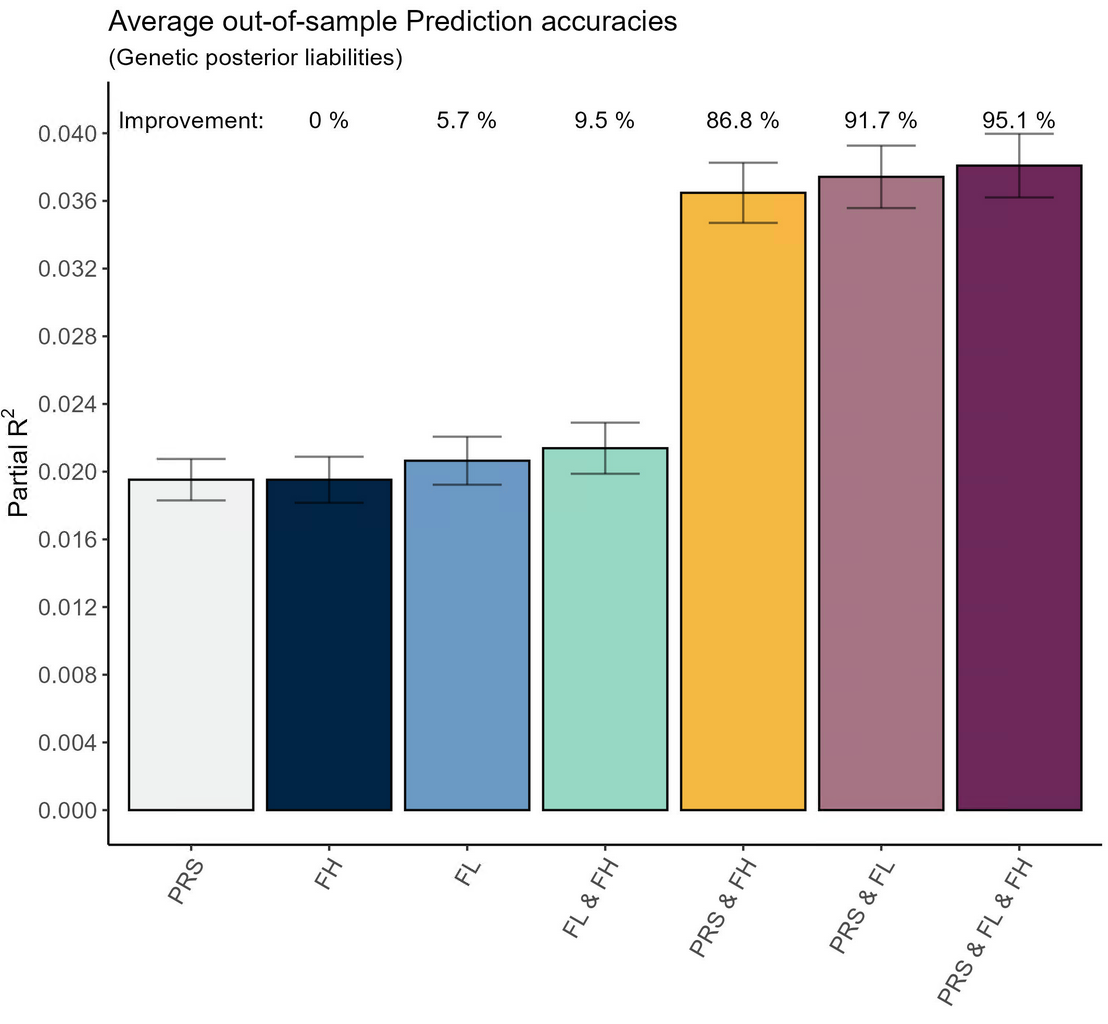
\includegraphics[width=10cm]{results/avg_partial_prediciton_accuracies_multi_trait.png}
	\caption[Average out of sample prediction for multi trait]{
		\sl Average partial $ R^2 $ across $ 5 $ disorders with various prediction models. The base model includes age, sex, and $ 20 $ PCs. As the prediction is based on multi trait, \textit{PRS} refers to the base model with the PRS of all considered phenotypes included. \textit{FH} refers to the base model with all binary family history variables included, and \textit{FL} refers to the model with all LT-FH++ variables included. Combinations of these variables are presented as \textit{PRS} \& \textit{FH} for the model with all PRSs and all binary family history variables etc..}
	\label{fig:paper3:predictionResultsMultiTrait}
\end{wrapfigure}

On top of this, we will also considered correlated phenotypes. Mental disorders are notoriously difficult to diagnose and many mental disorders have a high genetic correlation. Accounting for correlated phenotypes is therefore an attempt at utilising the information from the highly correlated phenotypes to improve prediction. For correlated trait, we restricted to the iPSYCH disorders. This was done due to the requirement of genetic correlations, which has already been calculated by Schork et al.\cite{schork2019genome}. In order to have as fair of a comparison as possible, we also created multi trait models for the other predictors. For instance, we considered a multi trait PRS model, which is a model with the PRS of all the considered correlated phenotypes. Similarly, the binary family history variable for all the correlated phenotypes was also included. For LT-FH++, we considered two scenarios. The first is the correlated phenotype extension as presented in \cref{sec:methods:ltfhpp:correlatedTraits}. It resulted in a single liability estimate that represents the family history for all of the considered disorders. We also considered a simpler approach, where the single trait LT-FH++ phenotype was included for each of the considered phenotypes. The first approach for LT-FH++ did not perform as well as the other methods, and will not be presented here. Therefore, we used the single trait LT-FH++ phenotype for each of the considered phenotypes. The multi trait results are presented in \cref{fig:paper3:predictionResultsMultiTrait}. 



When considering multiple traits, we did not observe any difference in predictive value between the considered PRSs and binary family history variables. The model with multiple single trait LT-FH++ phenotypes had a slightly higher predictive value, which was $ 5.7\% $ higher than the other two. As with the single trait prediction models, the model with both family history variables did not increase the predictive value, meaning most of the predictive value is captured by either of the family history variables. However, when considering a model with the multi trait PRS variables and either of the multi trait family history variables, we observe close to a doubling of the predictive value. This indicates that most of the predictive value caught by the PRS and family history models is different. The model with all three predictors has almost the same predictive value of the model with the PRS and either of the family history variables.


